\section{Durchführung}
\label{sec:Durchführung}

 Zunächst soll die Zeitkonstante eines RC-Gliedes bestimmt werden. Dazu wird die folgende Schaltung verwendet. Auf dem Oszilloskop soll nur die abfallende Flanke sichtbar sein; es wird dementsprechend eingestellt. Der Punkt an dem die Spannung Null ist (Minimum zwischen fallender und steigender Flanke), muss ausgemessen werden.

 \begin{figure}
   \centering
   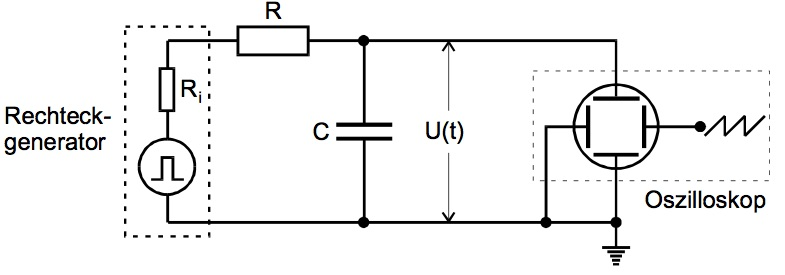
\includegraphics[scale=0.5]{content/messung_zeitkonstante.jpg}
   \caption{Schaltung zur Bestimmung der Zeitkonstante eines RC-Gliedes  Aus \cite{anleitung353}.}
   \label{fig:zeitkonstante}
 \end{figure}

Anschließend sollen die Kondensatorspannung sowie die Phasenverschiebung in Abhägigikeit der Frequenz untersucht werden. Die Generatorfrequenz wird zwischen 10 und 10000 \si{\Hz} erhöht. Es werden Werte der Frequenz, der Spannungsamplitude und der Phasenverschiebung aufgenommen.

\begin{figure}
  \centering
  \includegraphics[scale=0.5]{content/messung_frequenzabhängigkeit.jpg}
  \caption{Schaltung zur Messung der Kondensatorspannung in Abhängigkeit von der Frequenz. Aus \cite{anleitung353}.}
  \label{fig:kondensatorspannung}
\end{figure}

\begin{figure}
  \centering
  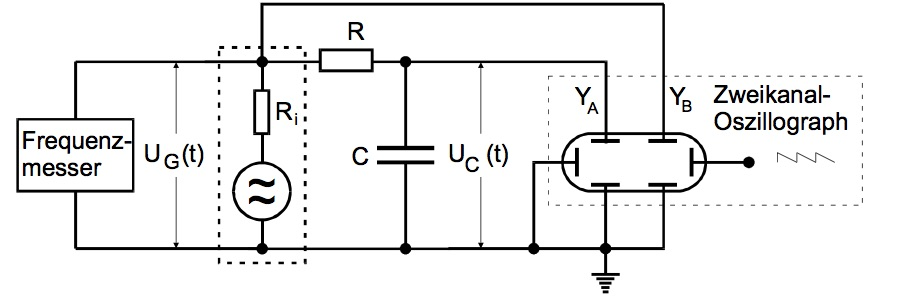
\includegraphics[scale=0.5]{content/messung_phasenverschiebung.jpg}
  \caption{Schaltung zur Messung der Phasenverschiebung zwischen Kondensator- und Generatorspannung in Abhängigkeit von der Frequenz. Aus \cite{anleitung353}.}
  \label{fig:phase-frequenz}
\end{figure}

Die Generatorspannung wird am Eingang $Y_A$ und die Kondensatorspannung an $Y_B$ angelegt. Dabei ist zu beachten, dass die Kurven der beiden Spannugsverläufe symmetrisch zur x-Achse sein müssen.
Ist die Phasenverschiebung größer Null, ist auf dem Oszilloskop etwa ein Bild wie in \ref{fig:phasenverschiebung} zu erkennen.

\begin{figure}
  \centering
  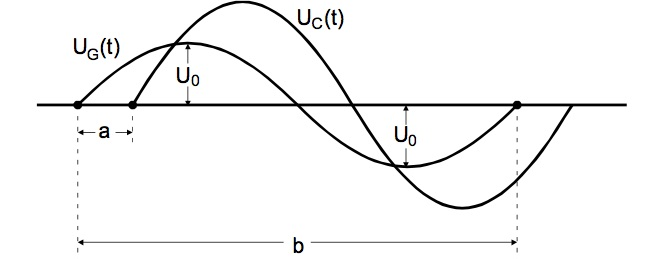
\includegraphics[scale=0.5]{content/Phasenverschiebung.jpg}
  \caption{Phasenverschiebung zwischen Kondensator- und Generatorspannung. Aus \cite{anleitung353}.}
  \label{fig:phasenverschiebung}
\end{figure}

Die Phasenverschiebung ergibt sich durch
\begin{equation}
  \phi = \frac{a}{b} \cdot 360 \quad\text{oder}\quad \phi = \frac{a}{b} \cdot 2\pi
\end{equation}

Um die Funktionsweise eines RC-Kreises als Integrator zu evaluieren, verwendet man die in \ref{fig:phase-frequenz} dargestellte Schaltung. Es sollen eine Rechteck-, Dreieck-, und Sinusspannung integriert werden. Die Kurve der Spannung soll sowohl vor als auch nach der Integration auf dem Oszilloskop dargestellt werden.
